\documentclass{ctexart}
\usepackage[utf8]{inputenc}
 % 插入MATLAB代码设置
\usepackage{caption}
\usepackage[dvipsnames]{xcolor} % 更全的色系
\usepackage{listings} % 排代码用的宏包
\usepackage{graphicx} 
\graphicspath{{img/}}  % 在当前目录下的figures文件夹下查找文件

\lstset{
	backgroundcolor = \color{yellow!10}, % 背景色:淡黄
	basicstyle = \small\ttfamily, % 基本样式 + 小号字体
	rulesepcolor= \color{gray}, % 代码块边框颜色
	breaklines = true, % 代码过长则换行
	numbers = left, % 行号在左侧显示
	numberstyle = \small, % 行号字体
	keywordstyle = \color{blue}, % 关键字颜色
	commentstyle =\color{red!100}, % 注释颜色
	stringstyle = \color{red!100}, % 字符串颜色
	frame = shadowbox, % 用(带影子效果)方框框住代码块
	showspaces = false, % 不显示空格
	columns = fixed, % 字间距固定
	%escapeinside={} % 特殊自定分隔符:
	morekeywords = {as} % 自加新的关键字(必须前后都是空格)
}

\title{\vspace{-2.5cm}Manderbrot Set 的生成和探索}
\author{顾格非 3210103528}
\date{\today}

\begin{document}
\maketitle  
\vspace{-0,5cm}
\begin{abstract}
曼德勃罗特集(Manderbrot Set)是一个几何图形,曾被称为“上帝的指纹”。本文摘要研究了曼德勃罗特集的一些性质,并通过计算机编程可视化了曼德勃罗特集。
\end{abstract}
\section{引言}
曼德博集合\cite{branner1989mandelbrot}(英语:Mandelbrot set,或译为曼德布洛特复数集合)是一种在复平面上组成分形的点的集合,以数学家本华·曼德博的名字命名。曼德博集合与朱利亚集合有些相似的地方,例如使用相同的复二次多项式来进行迭代。
\section{问题的背景介绍}
\subsection{定义}
对于每一个复数c,将迭代式$Z_{n+1}=Z_n^2+c$ 迭代无穷次,若得到的$Z_n$不发散到无穷大,把称这样的c在Mandelbrot集合中。将他们在复平面中画出来,就能得到图形\cite{stauffer1996newton}。

\section{数学理论}
若$c\in M,$则$|c|<=2$, 
若$c\in M,$则$|Z_n|\leq2,(n=1,2,3……)$

由于曼德布洛特集是一个封闭图形,且包含在以原点为中心,以2为半径的封闭圆盘中。故曼德布洛特集是一个紧集。

此外,杰里米 · 卡恩 Jeremy Kahn在2001年利用严格的拓扑证明,论证了曼德布洛特集的连通性。
由Adrien Douady和 John H. Hubbard证明曼德布洛特集连通时,所用到的曼德布洛特集的补集均匀化的动力学公式,引出了曼德布洛特集的外部尾迹射线。可将这些射线进行组合来研究曼德布洛特集,形成了 Yoccoz拼图的组合技术。
\newpage
\section{\vspace{-0.3cm}算法}
\subsection{伪代码呈现}
\begin{lstlisting}
  Choose a maximal iteration number N
  For each pixel p of the image:
  Let c be the complex number represented by p
  Let z be a complex variable
  Set z to 0
  Do the following N times:    
    If |z|>2 then color the pixel white, end this loop prematurely, go to the next pixel
    Otherwise replace z by z*z+c
  If the loop above reached its natural end: color the pixel p in black
  Go to the next pixel
\end{lstlisting}
\subsection{Python实现}
根据伪代码,我自己写了一个简单的程序,用二次循环遍历整个复平面,再用一次循环判断并调用第三方库画图。
\begin{lstlisting}[language=Python]
import numpy as np
import matplotlib.pyplot as plt
x = np.linspace(-2,2,800)
y = np.linspace(-2,2,600)
iter = 0
max_iter = 200 # 最终迭代次数
for a in x:
    for b in y:
        z = 0
        c = complex(a,b)
        for i in range(max_iter):
            z = z**2+c
            if abs(z)>2:
                break 
        if abs(z)<=2:
            plt.scatter(a,b,s=1,cmap='rainbow')
\end{lstlisting}

可以看到上面的算法之间用了三个for循环去遍历筛选,时间复杂度达到了$O(n^3)$,开销十分大。

而下面的Python代码记录了集合外的点跳出循环的次数,并将其与颜色建立一个映射,通过颜色的深浅表示出跳出循环的先后顺序。
\begin{lstlisting}[language=Python]
import numpy as np
import matplotlib.pyplot as plt
def iterator(c,r,max_iter):
    z=c #初始值
    for iter in range(0,max_iter,1):
        if abs(z)>r:break
        z=z**2+c
    return iter
def plot_mandelbrot(): #定义绘制mandelbrot图像
    X=np.linspace(-1.75,1.05,5000) #实部范围
    Y=np.linspace(-1.25,1.25,5000) #虚部范围
    real,image=np.meshgrid(X, Y) #生成网格点坐标矩阵。
    c=real+image*1j #构造复数
    mandelbrot_set = np.frompyfunc(iterator, 3, 1)(c, 1.5, 100).astype(np.float) #frompyfunc(func, nin, nout),
    plt.figure(dpi=500) #dpi设置分辨率
    plt.imshow(mandelbrot_set,extent=[-1.35, 1.35, -1.25, 1.25]);plt.show()
if __name_=="__main__":
    plot_mandelbrot()
\end{lstlisting}
\vspace{-0.5cm}
\begin{figure}[h]
	\centering
	\begin{minipage}{0.45\linewidth}
		\centering
		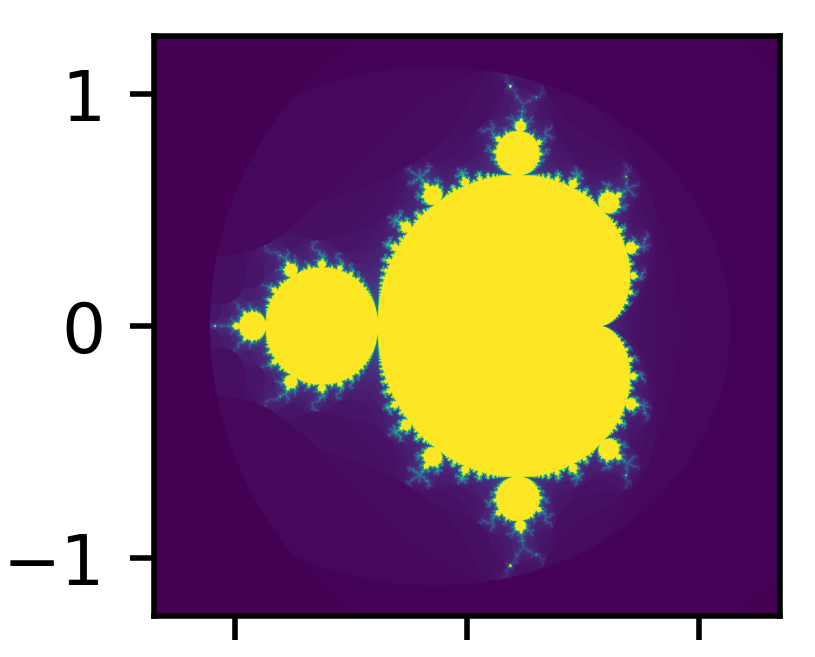
\includegraphics[width=0.92\linewidth]{Figure_1.png}
		\caption{\vspace{-0.7cm}Python的结果展示}
		\label{chutian1}%文中引用该图片代号
	\end{minipage}
	\begin{minipage}{0.45\linewidth}
		\centering
		\includegraphics[width=1.0\linewidth]{test.bmp}
		\caption{C++的结果展示}
		\label{chutian2}%文中引用该图片代号
	\end{minipage}
\end{figure}

\newpage
\section{数值算例}
经典的曼德勃罗集合采用的迭代式是$Z_{n+1}=Z_n^2+C$,这里我们尝试改变幂得到不同的迭代式,下面是得到的图形。虽然形状不同,但保留了自相似的性质。

\begin{figure}[htbp]
	\centering
	\begin{minipage}{0.4\linewidth}
		\centering
		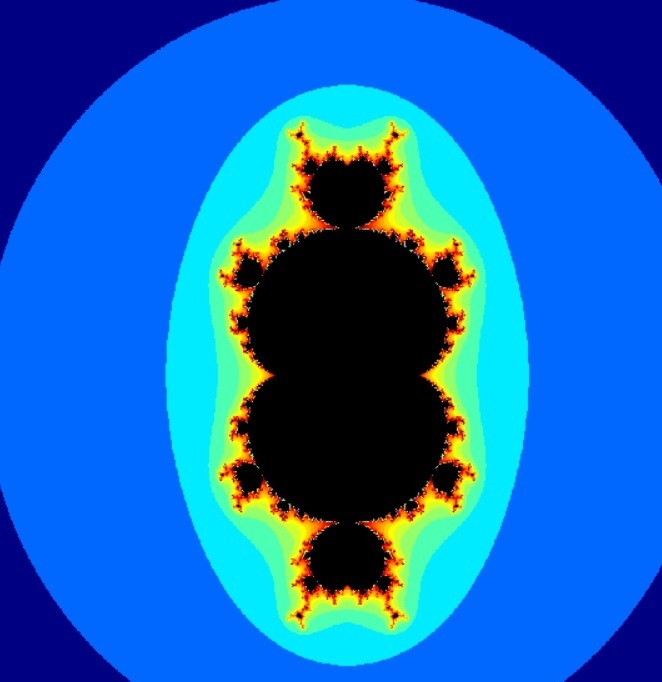
\includegraphics[width=0.52\linewidth]{1.jpg}	
		\caption{$Z_{n+1}=Z_n^3+C$}
		\label{chutian1}%文中引用该图片代号
	\end{minipage}
	%\qquad
	\begin{minipage}{0.52\linewidth}
		\centering
		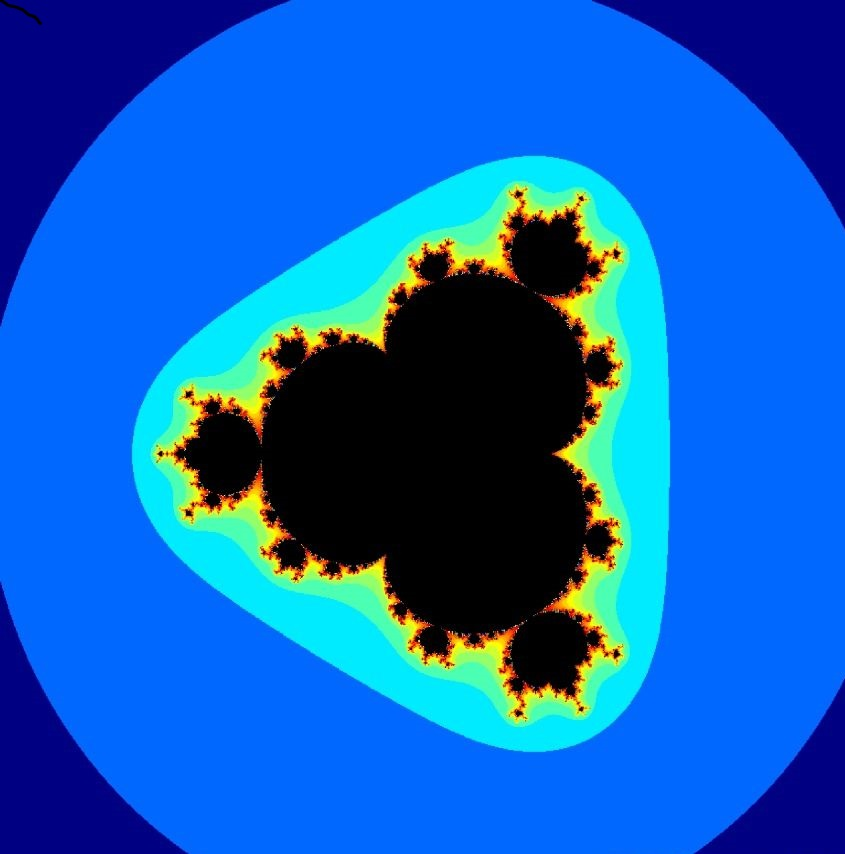
\includegraphics[width=0.42\linewidth]{2.jpg}
		\caption{$Z_{n+1}=Z_n^4+C$}
		\label{chutian2}%文中引用该图片代号
	\end{minipage}
\end{figure}
另外通过改变迭代次数,得到了不同精度的结果:(由于我们的算法判断条件是迭代次数到达$max\_iter$后,$|Z|<2$则认为在M集合内,且只要任何一个$Z_n>2$就break,所以随着$max\_iter$的增大,精度更高,图中黑色面积变小。
\begin{figure}[htbp]
	\centering
	\begin{minipage}{0.45\linewidth}
		\centering
		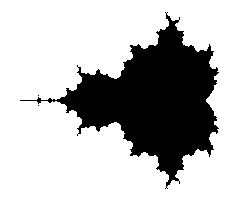
\includegraphics[width=0.62\linewidth]{M_iter_10.png}
		\caption{$max\_iter=10$}
		\label{chutian1}%文中引用该图片代号
	\end{minipage}
	%\qquad
	\begin{minipage}{0.45\linewidth}
		\centering
		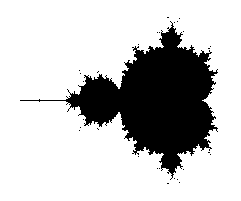
\includegraphics[width=0.62\linewidth]{M_iter_20.png}
		\caption{$max\_iter=20$}
		\label{chutian2}%文中引用该图片代号
	\end{minipage}
	\qquad
		\begin{minipage}{0.45\linewidth}
			\centering
			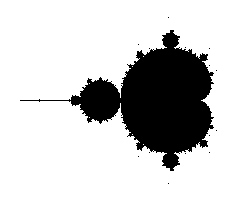
\includegraphics[width=0.62\linewidth]{M_iter_100.png}
			\caption{$max\_iter=100$}
			\label{chutian2}%文中引用该图片代号
		\end{minipage}
		\begin{minipage}{0.45\linewidth}
			\centering
			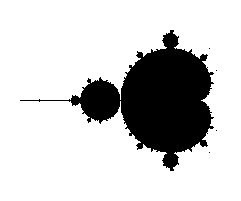
\includegraphics[width=0.62\linewidth]{M_iter_1E6.png}
			\caption{$max\_iter=1000000$}
			\label{chutian2}%文中引用该图片代号
		\end{minipage}
\end{figure}




\section{结论}
曼德勃罗集合十分神秘,虽然只是一个由简单的迭代式产生,但它具有优美的自相似性,让人体会到数学之美。

\bibliographystyle{plain}
\bibliography{ref}

\end{document}
